\chapter{Métricas de Evaluación de Imágenes}
\label{chap4}
\ifpdf
  \graphicspath{{Chapter4/Chapter4Figs/PNG/}{Chapter4/Chapter4Figs/PDF/}{Chapter4/Chapter4Figs/}}
\else
  \graphicspath{{Chapter4/Chapter4Figs/EPS/}{Chapter4/Chapter4Figs/}}
\fi

\markboth{\hfill \thechapter. Métricas de evaluación de imágenes}{\hfill \thechapter. Métricas de evaluación de imágenes}

% IQA (Image quality assessment)

Las imágenes digitales se ven afectadas por una amplia variedad de distorsiones durante la adquisición y procesamiento de este, que dan como resultado la pérdida de la calidad visual. La medición de la calidad visual es de suma importancia para diversas aplicaciones de procesamiento de imágenes y videos. 
 
Existen varios mecanismos para determinar la calidad de la imagen, generalmente asociados a una medida comparativa frente a una referencia. La mayoría de los enfoques existentes se basan en lo que se denomina \textbf{full reference} (FR) o {\it referencia completa}, lo que significa que se tiene acceso  completamente a la imagen original como referencia; el enfoque \textbf{non-reference} (NR) o {\it sin referencia}, en este enfoque no se requiere ningún acceso a la imagen original; y el enfoque \textbf{reduced reference} (RR) o {\it referencia reducida}, este enfoque no requiere un acceso total a la imagen original pero se necesita de alguna información parcial de referencia como por ejemplo un juego de características extraídas \cite{wang2004}. 

En esta sección se describen algunos enfoques de {\it referencia completa}.
Se realiza una selección de alternativas a partir de la necesidad de encontrar métricas que proporcionen el mejor balance entre mejora del contraste y distorsión.

Según el estado del arte, las métricas descritas a continuación son tradicionales, algunas más conocidas y utilizadas y otras son propuestas nuevas que demostraron su efectividad en cuanto a determinar la calidad de una imagen. 

De entre las métricas descritas hemos seleccionado 4 de ellas, para la propuesta de este trabajo. Las métricas seleccionadas serán parte de un estudio de correlación para determinar cuáles de ellas son eficientes para optimizar la elección de los parámetros en un sistema multiobjetivo.

\section{Error Cuadrático Medio (MSE)} 
\label{sec:mse}

El \textit{Error Cuadrático Medio} (\textit{MSE}, por sus siglas en inglés, Mean-Squared Error), se calcula promediando el cuadrado de la diferencia de intensidad entre píxeles distorsionados y de referencia \cite{wang2009}.

% Se supone que X e Y son dos señales discretas de longitud finita (por ejemplo, dos imágenes), donde N es el número de muestras (píxeles, en el caso de imágenes). El error cuadrático medio (MSE) entre dos imágenes es:

En el \textit{MSE}, nos referimos a la señal de error como la diferencia entre
la señal original y la señal distorsionada. Si partimos de que una de las señales es original o tiene calidad aceptable, entonces el \textit{MSE} puede ser visto como la medida de la calidad de la señal.

% $e_i = (f_{i} - {f'}_{i})$ señal de error;

Matemáticamente se lo define como:
\begin{equation}\label{eq:mse}
MSE(f,f') = \frac{1}{N}\sum_{i=1}^{N}(f_{i} - {f'}_{i})^{2}
\end{equation}

Donde: 
\begin{itemize} 
    \item f y f' : son imágenes;
    \item N: es el número de pixeles de cada imagen.
\end{itemize}


En la Figura \ref{fig:mse} se muestran ejemplos del \textit{MSE} de la imagen original \ref{fig:label:mse:1}, y sus imágenes modificadas \ref{fig:label:mse:2}, \ref{fig:label:mse:3}.

\begin{figure}[H]
    \begin{center}
        \subfigure[][\label{fig:label:mse:1}  $MSE=0$]{\includegraphics[width=4.5cm]{imagen2.png}}
        \subfigure[][\label{fig:label:mse:2} $MSE=14.9019$]{\includegraphics[width=4.5cm]{imagen2_1.png}}
        \subfigure[][\label{fig:label:mse:3} $MSE=2.5572$]{\includegraphics[width=4.5cm]{imagen2_1_ruido.png}}
    \end{center}
    \caption{Ejemplos de \textit{MSE} de imágenes médicas. \\
    (a) Imagen original.
    (b) Imagen mejorada usando el algoritmo \textit{CLAHE}.
    (c) Imagen contaminada por ruido.}
    \label{fig:mse}
\end{figure}


\section{Relación Señal a Ruido de Pico (PSNR)} 
\label{sec:psnr}

La \textit{Relación Señal a Ruido de Pico} (\textit{PSNR}, por sus siglas en inglés, Peak Signal-to-Noise Ratio). Es una función logarítmica del Error Cuadrático Medio \textit{MSE} \cite{annadurai2007fundamentals}.
% se mide en decibeles (dB)
Matemáticamente se lo define como:
% \begin{equation}\label{eq:psnr}
% PSNR = 10\log_{10} \frac{(2^b - 1)^2}{MSE}
% \end{equation}

\begin{equation}\label{eq:psnr}
PSNR = 10\log_{10} \frac{L^2}{MSE}
\end{equation}

Donde L, es el rango dinámico de las intensidades de pixeles de una imagen ($L = 2^b - 1$).

Por ejemplo, para imágenes que tienen asignaciones de 8 b/píxel de escala de grises, se tiene que $L = 2^8 - 1 = 255$.

Donde es el rango dinámico de la imagen. Por ejemplo, imágenes que utilizan 8 bits
por cada píxel, 

% El $PSNR$ es útil si se comparan imágenes que tienen diferentes rangos dinámicos, pero por lo demás no contiene información nueva relativa al $MSE$ \cite{wang2009}.


En la Figura \ref{fig:psnr} se muestran ejemplos del \textit{PSNR} de la imagen original \ref{fig:label:psnr:1}, y sus imágenes modificadas \ref{fig:label:psnr:2}, \ref{fig:label:psnr:3}.

\begin{figure}[H]
    \begin{center}
        \subfigure[][\label{fig:label:psnr:1} $PSNR=1000$]{\includegraphics[width=4.5cm]{imagen2.png}}
        \subfigure[][\label{fig:label:psnr:2} $PSNR=36.3984$]{\includegraphics[width=4.5cm]{imagen2_1.png}}
        \subfigure[][\label{fig:label:psnr:3} $PSNR=44.0332$]{\includegraphics[width=4.5cm]{imagen2_1_ruido.png}}
    \end{center}
    \caption{Ejemplos de \textit{PSNR} de imágenes médicas. \\
    (a) Imagen original.
    (b) Imagen mejorada usando el algoritmo \textit{CLAHE}.
    (c) Imagen contaminada por ruido.}
    \label{fig:psnr}
\end{figure}


\section{Índice de Similitud Estructural} 
\label{sec:ssim}

El \textit{Índice de Similitud Estructural} (\textit{SSIM}, por sus siglas en inglés, Structural Similarity Index) \cite{wang2004} fue desarrollado como un método para determinar la calidad de una imagen, es un coeficiente que mide el grado de distorsión producida en una imagen resultante $f'(i,j)$ a consecuencia de aplicar una \textit{Mejora del Contraste} a una imagen original o de referencia $f(i,j)$. 

Es una medida que pretende cuantificar de forma numérica y automática la calidad visual de una imagen para un observador humano, comparando entre la imagen original y reconstruida en cuanto a sus luminancias, contrastes e información de estructura. Proporciona un valor de calidad acotado entre 0 y 1. Un valor menor o cercano a cero significaría que la información de la estructura se ha perdido casi por completo.


El índice \textit{SSIM} aporta unos valores más cercanos a la realidad, ya que tiene un funcionamiento más cercano al comportamiento de la percepción humana \cite{wang2009}

% toma como premisa que el sistema visual humano está altamente adaptado a la extracción de información estructural de las escenas observadas

% El $SSIM$ nos da una idea de la distorsión que se ha producido en la estructura de la imagen y esto es lo que considera como la medida de la calidad que percibiría el observador.

El valor del \textit{SSIM} depende de tres factores claves: la luminancia (intensidad media), el contraste y la estructura. 
% Estas semejanzas locales se expresan usando medidas estadísticas y se combinan para formar el índice SSIM local.

Se hacen mediciones para cada componente fundamental de cada imagen, y posteriormente se realiza una comparación de cada componente de la imagen original con respecto al componente par de la imagen modificada, es decir, luminancia con luminancia, estructura con estructura y contraste con contraste. Por último, se realiza una combinación cuyo resultado determina el grado de similitud entre ambas. A mayor \textit{SSIM}, mayor similitud, que equivale a decir menor distorsión.

Siendo definidas dos imágenes digitales, $f$ representa a la imagen en su estado original y $f'$, representa a la imagen modificada por algún algoritmo cualquiera.

\begin{enumerate}
  \item \textbf{Luminancia} $l(f,f')$: La Luminancia, con respecto a la superficie del objeto imagen, depende de la iluminación y la reflectancia. Es un estimativo de la media de intensidades de gris. La función de comparación de luminancia es función de los promedios $\mu_f$ y $\mu_{f'}$. Por lo tanto, para comparar este factor, se define \textit{la media de intensidades} de gris de la imagen $f$ como $\mu_f$ \eqref{eq:media} y de la misma manera, la media de intensidades de gris de la imagen $f'$ como $\mu_{f'}$.

  \begin{equation}
    \label{eq:media}
    \mu_{f}=\frac{1}{M \times N}\sum_{i=1}^M \sum_{j=1}^N f(i,j)
  \end{equation}
    
  Se define la función de comparación de luminancia $l(f,f')$ como se ve en la función \eqref{eq:luminancia}, considerando que la variable $C_1$ es una constante, que se añade de manera a evitar inestabilidades, que pueden surgir cuando la suma entre $\mu_f^2$ y $\mu_{f'}^2$ es cercana a cero. Definamos a $C_1$ como sigue: $C_1 = (K_1 \times L)^2$, siendo $L$ el rango dinámico de valores de píxel, y $K_1 \ll 1$ es una constante pequeña; \\

  \begin{equation}
    l(f,f')=\frac{2\mu_f\mu_{f'}+C_1}{\mu_f^2+\mu_{f'}^2+C_1}
    \label{eq:luminancia}
  \end{equation}

  \item \textbf{Contraste} $c(f,f')$: La variación de contraste entre imágenes depende de las desviaciones típicas de ambas, por tanto se debe calcular la desviación $\sigma_f$ de la imagen $f$ mediante la expresión \eqref{eq:desviacion} y de la misma manera $\sigma_{f'}$ para la imagen $f'$. La función de comparación de contraste es entonces una comparación de $\sigma_f$ y $\sigma_{f'}$.

    \begin{equation}
        \label{eq:desviacion}
        \sigma_{f}=\sqrt{\frac{1}{(M \times N)-1}\sum_{i=1}^M\sum_{j=1}^N(f_{(i,j)}-\mu_f)^2}
    \end{equation}

    La función de comparación de contraste $c(f,f')$ se define como se muestra en la función \eqref{eq:terminocontraste}, donde $C_2=(K_2 \times L)^2$, el cual tiene los mismos parámetros que se definieron para $C_1$.

    \begin{equation}
        c(f,f')=\frac{2\sigma_f\sigma_{f'}+C_2}{\sigma_f^2+\sigma_{f'}^2+C_2}
        \label{eq:terminocontraste}
    \end{equation}

    \item \textbf{Estructura} $s(f,f')$: Para definir la información estructural de una imagen, se buscan las características que definen la representación de los objetos que componen la escena, de forma independiente de la luminancia y el contraste. La comparación de estructura está compuesta por la covarianza $\sigma_{ff'}$ y las desviaciones típicas $\sigma_f$ y $\sigma_{f'}$. Por lo tanto, es necesario calcular la covarianza entre las imágenes $f$ y $f'$ como se muestra en la expresión \eqref{eq:covarianza}.
    
    \begin{equation}\label{eq:covarianza}
        \sigma_{ff'}=\frac{1}{(M \times N)-1}\sum_{i=1}^M\sum_{j=1}^N(f_{(i,j)}-\mu_f)({f'}_{(i,j)}-\mu_{f'})
    \end{equation}
    
    La covarianza indica que tanto se asemejan las estructuras de píxeles entre las dos imágenes, es decir, si es positiva hay semejanza entre las estructuras y si es negativa hay diferencia entre las estructuras. De esta manera, el término de información estructural $s(f,f')$ se define como se muestra en la función \eqref{eq:informacionestructural}:
    
    \begin{equation}
        s(f,f')=\frac{\sigma_{ff'}+C_3}{\sigma_f\sigma_{f'}+C_3}
        \label{eq:informacionestructural}
    \end{equation}
\end{enumerate}

En \eqref{eq:media}, \eqref{eq:desviacion} y \eqref{eq:covarianza} cada elemento $f(i,j)$ de la matriz representa a un píxel de la imagen con $i=\{1,2,...,M\}$ y $j=\{1,2,...,N\}$.

% Las estadísticas descritas anteriormente se calculan localmente, obteniendo un $SSIM$ local para cada punto de la imagen desplazando una ventana gaussiana. Se tendría así un mapa de cómo varía espacialmente la calidad y de este mapa se obtiene un SSIM global haciendo simplemente la media.

En la Figura \ref{fig:ssim_elementos} se muestra la combinación de los tres componentes para dar la medida de similitud $SSIM$ dada en la expresión \eqref{eq:ssimgeneral}

\begin{figure} [H]
\centering
\resizebox{10.5cm}{10cm}{
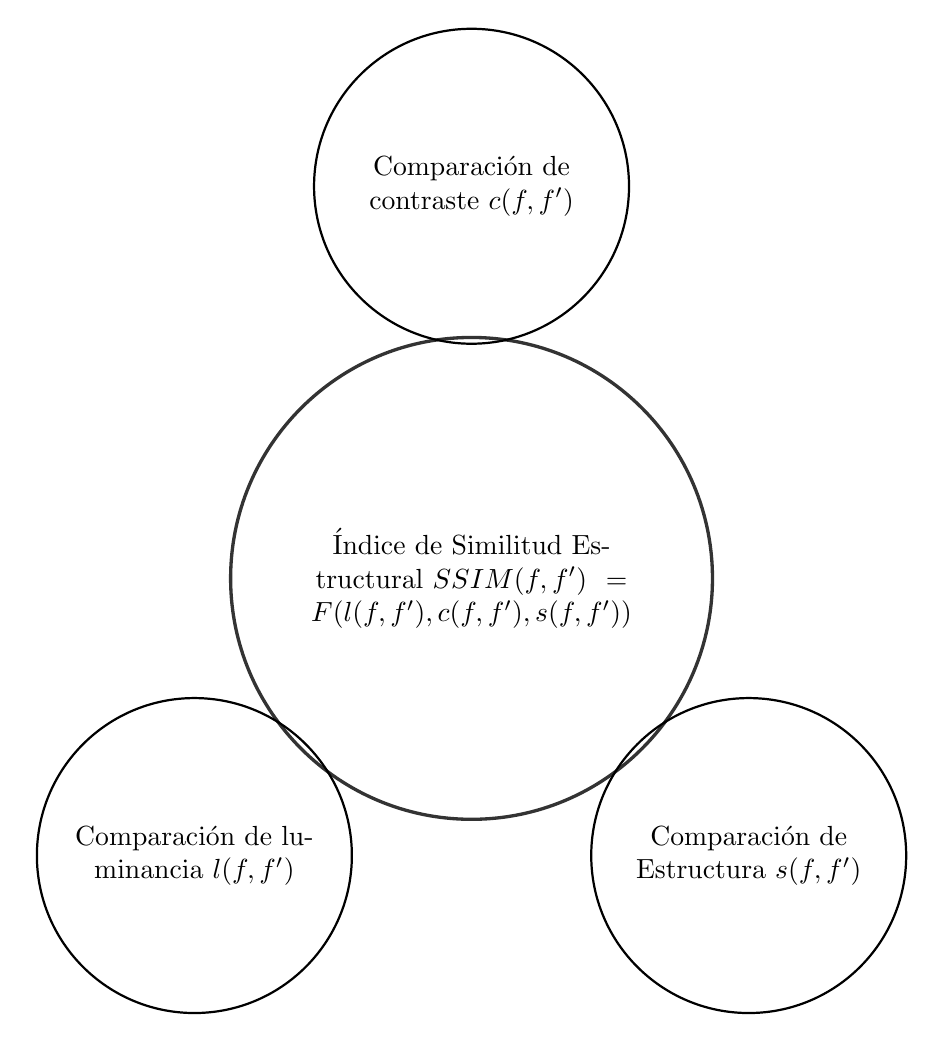
\begin{tikzpicture}[thick]
\node [circle, draw=black!80, very thick, inner sep=0pt, minimum size=4.6cm, text width=6cm,align=center] (1) at (2,2) {Índice de Similitud Estructural $SSIM(f,f')=F(l(f,f'),c(f,f'),s(f,f'))$};
\draw (2,6.98) circle (2cm) node[text width=4cm,align=center] {Comparación de contraste $c(f,f')$};
\draw (-1.52,-1.52) circle (2cm) node[text width=4cm,align=center] {Comparación de luminancia $l(f,f')$};
\draw (5.52,-1.52) circle (2cm) node[text width=3.5cm,align=center] {Comparación de Estructura $s(f,f')$};
\end{tikzpicture}
}

\caption{Diagrama de elementos componentes del Índice de Similitud Estructural.}
\label{fig:ssim_elementos}
\end{figure}

Las funciones $l(f,f')$, $c(f,f')$ y $s(f,f')$ se han desarrollado de forma a que cumplan las tres condiciones siguientes \cite{wang2004}:

\begin{itemize}
\item Simetría: $SSIM(f,f')=SSIM(f',f)$ 
\item Límite: $SSIM(f,f') \leqslant  1$ 
\item Máximo único: $SSIM(f,f')=1$ si y solo si $f=f'$
\end{itemize}

Al utilizar conjuntamente las tres ecuaciones \ref{eq:luminancia}, \ref{eq:terminocontraste} y \ref{eq:informacionestructural}, se define de forma general el \textit{Índice de Similitud Estructural} entre dos imágenes $f$ y $f'$ según la Ecuación \ref{eq:ssimgeneral}.

\begin{equation}
SSIM(f,f')==[l(f,f')]^\alpha+[c(f,f')]^\beta+[s(f,f')]^\gamma
\label{eq:ssimgeneral}
\end{equation}

Donde:
\begin{itemize}
\item $\alpha=\beta=\gamma=1$;
\item $C_3=\frac{C_2}{2}$; 
\item $\alpha$, $\beta$ y $\gamma$ definen el grado de prioridad de cada componente.
\end{itemize}

\begin{equation}\label{eq:ssim}
    SSIM(f,f')=\frac{(2\mu_f\mu_{f'}+C_1)(2\sigma_{ff'}+C_2)}{(\mu_f^2+\mu_{f'}^2+C_1)(\sigma_f^2+\sigma_{f'}^2+C_2)} \quad SSIM \in [0,1]
\end{equation}

Donde:
\begin{itemize}
\item $\mu_f$ es el promedio de intensidades de $f$;
\item $\mu_f'$ es el promedio de intensidades de $f'$; 
\item $\sigma_f^2$ y $\sigma_{f'}^2$ son las varianzas de intensidades de $f$ e $f'$, respectivamente;
\item $\sigma_{ff'}$ es la covarianza entre $f$ e $f'$;
\item $C_1=(K_1L^2)$, $K_1 \ll 1$ es una constante pequeña;
\item $C_2=(K_2 L)^2$, y $K_2 \ll 1$;
\item tanto $C_1$ y $C_2$ son constantes que se usan para estabilizar la división en caso de que el denominador tienda a cero.
\end{itemize}

% \textit{SSIM} se calcula por bloques, como resultado se obtiene un conjunto de coeficientes $SSIM$, donde cada $SSIM$ corresponde a un sector procesado. Sin embargo, en la práctica se necesita de que el coeficiente \textit{SSIM} sea único y que permita evaluar la distorsión de una imagen original respecto a su modificación en su totalidad y no por sectores. Por ello, el resultado final de la métrica es la media de todos los coeficientes \textit{SSIM} resultantes calculados en cada sector de la imagen.

Entre las ventajas de este método cabe destacar su sencillez, portabilidad, robustez y escaso costo computacional. 

\textit{SSIM} se ha utilizado para evaluar los resultados del procesado de imágenes en un creciente número de aplicaciones, como por ejemplo, fusión de imágenes, compresión de imágenes, transmisión (streaming) de video inalámbrico, vigilancia, imágenes de radar, imágenes de infrarrojo, imagen de resonancia magnética (MRI), reconocimiento de objetos.

% La función ssim devuelve el mapa SSIM que supone la comparación píxel a píxel entre las dos imágenes.

En la Figura \ref{fig:ssim} se muestran ejemplos del \textit{SSIM} de la imagen original \ref{fig:label:ssim:1}, y sus imágenes modificadas \ref{fig:label:ssim:2}, \ref{fig:label:ssim:3}.

\begin{figure}[H]
    \begin{center}
        \subfigure[][\label{fig:label:ssim:1} $SSIM=1$]{\includegraphics[width=4.5cm]{imagen2.png}}
        \subfigure[][\label{fig:label:ssim:2} $SSIM=0.7978$]{\includegraphics[width=4.5cm]{imagen2_1.png}}
        \subfigure[][\label{fig:label:ssim:3} $SSIM=0.4837$]{\includegraphics[width=4.5cm]{imagen2_1_ruido.png}}
    \end{center}
     \caption{Ejemplos de \textit{SSIM} de imágenes médicas. \\
    (a) Imagen original.
    (b) Imagen mejorada usando el algoritmo \textit{CLAHE}.
    (c) Imagen contaminada por ruido.}
    \label{fig:ssim}
\end{figure}

\section{Índice de Similitud de Características (FSIM)} 
\label{sec:fsim}

El \textit{Índice de Similitud de Características} (\textit{FSIM}, por sus siglas en inglés, Feature Similarity Index), se basa en el hecho de que el sistema visual humano, ($HVS$, por sus siglas en inglés, Human Visual System), comprende una imagen principalmente según sus características de bajo nivel. Utiliza la congruencia de fase ($PC$, por sus siglas en inglés, Phase Congruency), que es una medida adimensional de la importancia de una estructura local. Teniendo en cuenta que la $PC$ es invariante de contraste, mientras que la información de contraste afecta la percepción de $HVS$ de la calidad de imagen y la magnitud del gradiente de imagen ($GM$, por sus siglas en inglés, Gradient Magnitude), ambos juegan roles complementarios en la caracterización de la calidad local de la imagen \cite{fsim2011}.

% la congruencia de fase (PC) y la magnitud de gradiente (GM) se utilizan en FSIM y representan aspectos complementarios de la calidad visual de la imagen. El valor de PC también se usa para ponderar la contribución de cada punto a la similitud general de dos imágenes.
% Después de obtener el mapa de calidad local, usamos PC nuevamente como una función de ponderación para derivar un puntaje de calidad único.
% FSIM está diseñado para imágenes en escala de grises, la información de crominancia puede incorporarse fácilmente por medio de una simple extensión de FSIM, y llamamos a esta extensión FSIMC.


Matemáticamente se lo puede definir como:
\begin{equation}\label{eq:fsim}
FSIM (i,j) = S_{GM}(i,j) S_{PC}(i,j)
\end{equation}

Donde: 
\begin{itemize}
\item $S_{GM}(i,j)$ y  $S_{PC}(i,j)$ son medidas de similitud de la medida del gradiente y la congruencia de fase respectivamente, y se definen como sigue:
\end{itemize}

% is a commonly used measure to define the similarity of two positive real numbers and its result ranges within (0-1].
\begin{equation}\label{eq:sgm}
S_{GM}(i,j) = \frac{2G_f(i,j)G_{f'}(i,j)+T1}{G_{f}^{2}(i,j) + G_{f'}^{2}(i,j)+T1}
\end{equation}

\begin{equation}\label{eq:spc}
S_{PC}(i,j) = \frac{2PC_f(i,j)PC_{f'}(i,j)+T1}{PC_{f}^{2}(i,j) + PC_{f'}^{2}(i,j)+T1}
\end{equation}

Donde: 
\begin{itemize}
\item $f$ y $f'$ son las imágenes de referencia y la modificada.
\item T1 y T2 son constantes positivas.
\end{itemize}

En la Figura \ref{fig:fsim} se muestran ejemplos del \textit{FSIM} de la imagen original \ref{fig:label:fsim:1}, y sus imágenes modificadas \ref{fig:label:fsim:2}, \ref{fig:label:fsim:3}.

\begin{figure}[H]
    \begin{center}
        \subfigure[][\label{fig:label:fsim:1}  $FSIM=1$]{\includegraphics[width=4.5cm]{imagen2.png}}
        \subfigure[][\label{fig:label:fsim:2}  $FSIM=0.8046$]{\includegraphics[width=4.5cm]{imagen2_1.png}}
        \subfigure[][\label{fig:label:fsim:3}  $FSIM=0.8073$]{\includegraphics[width=4.5cm]{imagen2_1_ruido.png}}
    \end{center}
    \caption{Ejemplos de \textit{FSIM} de imágenes médicas. \\
    (a) Imagen original.
    (b) Imagen mejorada usando el algoritmo \textit{CLAHE}.
    (c) Imagen contaminada por ruido.}
    \label{fig:fsim}
\end{figure}


\section{Índice de similitud de gradientes (GSIM)} 
\label{sec:gsim}

El \textit{Índice de similitud de gradientes} (\textit{GSIM}, por sus siglas en inglés, Gradient Similarity Index), mide los cambios en el contraste y la estructura en las imágenes. Al igual que el $SSIM$ considera tanto la luminancia como los cambios estructurales de contraste para evaluar de manera efectiva la calidad de la imagen \cite{gsim2012}.

El gradiente de una imagen es un cambio direccional en la intensidad o el color de la imagen. Los gradientes de la imagen se pueden usar para extraer información de esta; transmiten información visual importante y son cruciales para entender la escena.

%Usando tal información, los cambios estructurales y de contraste pueden ser capturados efectivamente.
% En el software de gráficos para edición digital de imágenes, el término gradiente se usa para una combinación gradual de color que puede considerarse como una gradación uniforme de valores bajos a altos, tal como se usa de blanco a negro en las imágenes de la derecha.

El gradiente en cada punto de la imagen es un vector 2D con los componentes dados por las derivadas en las direcciones horizontal y vertical. En cada punto de imagen, el vector de gradiente apunta en la dirección del mayor aumento de intensidad, y la longitud del vector de gradiente corresponde a la velocidad de cambio en esa dirección.

% El gradiente de la imagen es uno de los bloques de construcción fundamentales en el procesamiento de imágenes. Los gradientes de imagen a menudo se utilizan en mapas y otras representaciones visuales de datos para transmitir información adicional. Las herramientas GIS usan progresiones de color para indicar elevación y densidad de población, entre otras.

Matemáticamente se define como:
\begin{equation}\label{eq:gradiente}
g(f,f') = \frac{2g_f g_{f'}+ C4} {g_f^{2} g_{f'}^{2} + C4}
\end{equation}

Donde: 
\begin{itemize}
\item $g_f$ y  $g_{f'}$ son los valores del gradiente lo largo de las imágenes $f$ y $f'$.
\item $C4$  es una constante positiva, para evitar que el denominador sea cero.
\item $g(f,f')$ es la similitud de gradiente entre  $f$ y $f'$, y su valor se encuentra en [0, 1]
\end{itemize}

En la Figura \ref{fig:gsm} se muestran ejemplos del \textit{GSIM} de la imagen original \ref{fig:label:gsm:1}, y sus imágenes modificadas \ref{fig:label:gsm:2}, \ref{fig:label:gsm:3}.

\begin{figure}[H]
    \begin{center}
        \subfigure[][\label{fig:label:gsm:1} $GSIM=1$]{\includegraphics[width=4.5cm]{imagen2.png}}
        \subfigure[][\label{fig:label:gsm:2} $GSIM=0.9772$]{\includegraphics[width=4.5cm]{imagen2_1.png}}
        \subfigure[][\label{fig:label:gsm:3} $GSIM=0.9781$]{\includegraphics[width=4.5cm]{imagen2_1_ruido.png}}
    \end{center}
    \caption{Ejemplos de \textit{GSIM} de imágenes médicas. \\
    (a) Imagen original.
    (b) Imagen mejorada usando el algoritmo \textit{CLAHE}.
    (c) Imagen contaminada por ruido.}
    \label{fig:gsm}
\end{figure}


\section{Local Tuned Global Model (LTG)}
\label{sec:ltg}
El modelo \textit{Local Tuned Global (LTG)} fue introducido bajo la hipótesis de que la percepción visual humana en la calidad de la imagen depende de la distorsión local resaltante y la degradación global de la calidad \cite{ltg2014}. 

\textit{LTG} es un enfoque basado en el gradiente de la imagen, ya que ésta es muy sensible a las distorsiones de la misma; así también extrae información sobre la luminancia (brillo percibido por el ojo humano) y la crominancia (información del color) de la imagen de entrada y la imagen distorsionada, luego mide la distorsión local resaltante y la degradación global de la calidad en la información obtenida sobre la luminancia y compara las diferencias en la información obtenida sobre la crominancia, derivando así el valor global de la calidad de la imagen \cite{jahne1999handbook}.
 
El gradiente $GM$ es una aproximación de la derivada de primer orden de la función de la imagen. Se utiliza para acentuar detalles y bordes de una imagen, es un método muy utilizado para la detección de bordes de una imagen. El gradiente de una imagen mide cómo ésta cambia en términos de intensidad. La magnitud del gradiente nos indica la rapidez con la que la imagen está cambiando, mientras que la dirección del gradiente nos indica la dirección en la que la imagen está cambiando más rápidamente \cite{esquedagradiente}.

La magnitud del gradiente $GM$ para una imagen $f$ está definida por:

\begin{equation}\label{eq:gm}
G = \sqrt[]{G_{h}^{2} + G_{v}^{2}}
\end{equation}

Donde: 
\begin{itemize}
\item $G_{h}$ y  $G_{v}$ son las derivadas parciales de la imagen a lo largo de las direcciones horizontal y vertical utilizando el operador Scharr \cite{jahne1999handbook}.
\end{itemize}
 

El gradiente de la fila $G_h$ y de columna $G_v$ en cada píxel se obtiene mediante la convolución de la imagen $f$ con las máscaras H y V (\ref{scharr}), esto es: 


\begin{equation}\label{gh}
    G_h(i,j) = f(i,j) \otimes{} H(i,j)
\end{equation}

\begin{equation}\label{gv}
    G_v(i,j) = f(i,j) \otimes{} V(i,j)
\end{equation}

Las máscaras utilizadas para las direcciones horizontal y vertical, se definen como:

\begin{equation}\label{scharr}
  H = \frac{1}{16} = \left\{{\begin{tabular}{ccc}
  3 & 0 & -3 \\
  10 & 0 & -10 \\
  3 & 0 & -3 
  \end{tabular}}\right\} 
  V = \frac{1}{16} = \left\{{\begin{tabular}{ccc}
  3 & 10 & 3 \\
  0 & 0 & 0 \\
  -3 & -10 & -3 
  \end{tabular}}\right\}
\end{equation}

En la Figura \ref{fig:gradiente} se muestra el gradiente de una imagen.
\begin{figure}[H]
  \begin{center}
    \leavevmode
    \includegraphics[height=6cm]{gradiente_imagen1_invertida}
    \caption{Ejemplo del Gradiente de una imagen médica.}
    \label{fig:gradiente}
  \end{center}
\end{figure}

Para detectar la diferencia de los mapas de $GM$ de la imagen original $f$ y su versión modificada $f'$ se calcula:

\begin{equation}\label{eq:gm_1}
G_m(f,f') = \frac{2G_{f}  * G_{f'} + C_1}{G_{f}^{2}+G_{f'}^{2}+C_1} 
\end{equation}

Donde:
\begin{itemize}
\item $G_{f}$ y $G_{f'}$ son los gradientes de la imagen original $f$ y la imagen modificada $f'$;
\item $C_1$ es una constante positiva;
\item $G_{m}$ es el gradiente medio de la imagen original y modificada.
\end{itemize}

% Gm logra capturar la notable distinción entre las imágenes originales y distorsionadas.

Una vez calculado el mapa de $GM$, se halla un promedio global utilizando la siguiente formula:
 
\begin{equation}\label{eq:gg}
G_g(f,f') = \Phi (G_m) = \frac{1}{M} \sum_{i=1}^{M}G_m(f_i,{f'}_i)
\end{equation}

Donde:
\begin{itemize}
\item $M$ es el número total de píxeles en la imagen;
\item $\Phi$ calcula el valor medio.
\end{itemize}

% La agrupación global promedio funciona de manera ineficaz, ya que disminuye seriamente la influencia de las distorsiones locales sobresalientes sobre la calidad de la imagen, y por lo tanto deriva una calificación no razonable.

% En general, los ojos humanos fijan algunas regiones destacadas antes de escanear toda la imagen. Esas regiones salientes se pueden considerar aproximadamente como las áreas que son en gran parte distintas del entorno.

Para las distorsiones locales, se ajusta el promedio global para un mejor rendimiento y poder enfatizar las regiones de alta distorsión, se define la siguiente formula:
\begin{equation}\label{eq:gl}
G_l(f,f') = \Phi (G_s)=\frac{1}{M_s} \sum_{i=1}^{M_s} G_s(f_i,{f'}_i)
\end{equation}

Donde:
\begin{itemize}
\item $ G_{s}$ indica los píxeles con valores $s\%$ más altos en $G_{m}$;
\item $M_s$ es el número de píxel en $G_s$
% En esta implementación se asigna a s=15.
\end{itemize}


Antes del cálculo del $GM$ se utiliza el modelo de color $YIQ$, ampliamente utilizado en el procesamiento de imágenes, ($Y$ es el canal de luminancia o brillo; $I$ es el canal para fase de entrada del color y $Q$ es el canal para cuadratura del color), para transferir una imagen RGB de entrada utilizando:

% $YIQ$: fue diseñado para aprovechar la mayor sensibilidad del sistema visual humano a los cambios de la saturación. La ventaja en el procesamiento de imágenes es que la luminancia (Y) y la información del color (I y Q) están desacoplados, así la componente de luminancia (y) puede procesarse sin afectar su contenido cromático.


\begin{equation}\label{eq:yiq}
\begin{bmatrix}
Y\\ 
I\\ 
Q
\end{bmatrix} = \begin{bmatrix}
0.299 &  0.587 & 0.114\\ 
 0.596 & -0.275 & -0.321\\ 
 0.212 & -0.523 & 0.311
\end{bmatrix} \begin{bmatrix}
R\\ 
G\\ 
B
\end{bmatrix}
\end{equation}

$Y$ (información de luminancia), se utiliza en el cálculo de $G_l$ (ecuación \ref{eq:gl}) y $G_g$ (ecuacón \ref{eq:gg}). $I$ y $Q$ (información del color) se utilizan para medir la diferencia de crominancia entre las imágenes original $f$ y modificada $f'$ , utilizando las siguientes formulas:


\begin{equation}\label{eq:gm_3}
I_m(f,f') = \frac{2I_f*I_{f'}+C_2}{I_{f}^{2}+I_{y}^{2}+C_2} 
\end{equation}
\begin{equation}\label{eq:gm_4}
Q_m(f,f') = \frac{2Q_f*Q_{f'}+C_2}{Q_{f}^{2}+Q_{f'}^{2}+C_2} 
\end{equation}

Donde:
\begin{itemize}
\item $I_f$ y $I_{f'}$, ($Q_f$ y $Q_{f'}$) contienen la información de crominancia de las imágenes $f$ y $f'$;
\item $C_2$ es una constante positiva;
\end{itemize}

Finalmente, el $LTG$ propuesto combina ambas partes:

\begin{equation}\label{eq:ltg}
LTG(f, f') = \frac{\Phi(G_{s}^{\theta_1})}{\Phi(G_{m}^{\theta_2})} \Phi(I_{m}^{\theta_3}.Q_{m}^{\theta_3})
\end{equation}

Donde, $\theta_1$ a $\theta_3$ ( $\theta_1 > \theta_2$ ) son parámetros del modelo.

En la Figura \ref{fig:ltg} se muestran ejemplos del $LTG$ de la imagen original \ref{fig:label:ltg:1}, y sus imágenes modificadas \ref{fig:label:ltg:2}, \ref{fig:label:ltg:3}.

\begin{figure}[H]
    \begin{center}
        \subfigure[][\label{fig:label:ltg:1} $LTG=1$]{\includegraphics[width=4.5cm]{imagen2.png}}
        \subfigure[][\label{fig:label:ltg:2} $LTG=0.8921$]{\includegraphics[width=4.5cm]{imagen2_1.png}}
        \subfigure[][\label{fig:label:ltg:3} $LTG=0.8358$]{\includegraphics[width=4.5cm]{imagen2_1_ruido.png}}
    \end{center}
    \caption{Ejemplos de $LTG$ de imágenes médicas. \\
    (a) Imagen original.
    (b) Imagen mejorada usando el algoritmo $CLAHE$.
    (c) Imagen contaminada por ruido.}
    \label{fig:ltg}
\end{figure}



\section{Entropía} 
\label{sec:entropia}

La Entropía de la Información es un concepto definido originalmente por Shannon \cite{shannon}, que busca un método de medición de la información proporcionada por un evento determinado, mide que tan bien se utilizan los niveles de gris disponibles en una imagen.

Para el cálculo de la \textit{Entropía} en imágenes médicas, se hace uso de la distribución de los niveles de grises de la imagen, estimando la distribución de probabilidades para los valores de grises contando el número de veces que un nivel de gris aparece en la imagen y dividiéndolo por el total de ocurrencias. Una imagen que contenga casi solo un mismo nivel de gris proporcionará poca información, tendrá una baja entropía a diferencia de una imagen que posea cantidades relativamente similares de una serie de niveles de grises \cite{gimenezlopez}.

Al comparar imágenes es importante tener algún tipo de medida sobre la cantidad de información disponible en dichas imágenes. La \textit{Entropía} nos indica la riqueza de los detalles de una imagen. Cuanto más cercano sea el valor de la entropía de la imagen resultante con respecto a la imagen original, se puede decir que los detalles de la imagen se han conservado \cite{daumasjara}.

En el contexto de la mejora de contraste, podemos afirmar que la información contenida en una imagen aumenta como consecuencia del aprovechamiento de los niveles de gris disponibles para la representación de la misma, por tanto, al maximizar la \textit{Entropía} de la imagen, también se aumenta el contraste que posee \cite{daumasjara} ya que la métrica está fuertemente asociada al brillo medio de la imagen \cite{108593}. Maximizar la \textit{Entropía} consiste en lograr que la imagen tenga un histograma más uniforme, donde cada nivel de gris posee la misma probabilidad de ocurrencia.

Matemáticamente se lo define como:
\begin{equation}\label{eq:entropia}
\mathscr{H}=-\sum_{k=0}^{L-1}\mathcal{P}_k log_2(\mathcal{P}_k)  \quad \mathscr{H} \in \left[0,log_2(L-1) \right]
\end{equation}


Donde: 
\begin{itemize} 
    \item $\mathcal{P}_k=\frac{n_k}{Z}$, donde $n_k$ es la cantidad de ocurrencias del i-ésimo nivel de gris y $Z$ la cantidad total de píıxeles, en el histograma;
    \item $L-1$ es el máximo nivel de gris que se puede utilizar para representar la imagen
\end{itemize}

La razón por la que se utiliza logaritmo en base 2 es que tratamos con imágenes digitalizadas en nuestro estudio.

La \textit{Entropía} por sí sola no es suficiente para determinar si la mejora de contraste realizada es satisfactoria, debido a que no cuantifica la amplificación del ruido ni la distorsión o degradación en la estructura de una imagen como consecuencia de aplicar $CLAHE$ \cite{morebrizuela2014}.

En la Figura \ref{fig:entropia} se muestran ejemplos de la \textit{Entropía} de la imagen original \ref{fig:label:entro1}, y sus imágenes modificadas \ref{fig:label:entro2}, \ref{fig:label:entro3}.

\begin{figure}[H]
    \begin{center}
        \subfigure[][\label{fig:label:entro1} $\mathscr{H}=6.6690$]{\includegraphics[width=4.5cm]{imagen2.png}}
        \subfigure[][\label{fig:label:entro2} $\mathscr{H}=7.1386$]{\includegraphics[width=4.5cm]{imagen2_1.png}}
        \subfigure[][\label{fig:label:entro3} $\mathscr{H}=6.6969$]{\includegraphics[width=4.5cm]{imagen2_1_ruido.png}}
    \end{center}
    \caption{Ejemplos de \textit{Entropía} de imágenes médicas. \\
    (a) Imagen original.
    (b) Imagen mejorada usando el algoritmo $CLAHE$.
    (c) Imagen contaminada por ruido.}
    \label{fig:entropia}
\end{figure}


\section{Entropía Local}
\label{sec:entropialocal}

La \textit{Entropía Local} \cite{localentropy} está relacionada con la variación de los niveles de gris en la vecindad de un pixel. Divide la imagen en bloques y luego analiza cada región como fuente de información separada.

La \textit{Entropía Local} mide la aleatoriedad de la imagen calculando la media de la muestra de la \textit{Entropía} sobre una serie de bloques no superpuestos de la imagen y seleccionados al azar, debido a esto es capaz de superar algunas debilidades conocidas de la Entropía de Shannon \cite{localshanonentropy}.

\begin{itemize}
 \item A diferencia de la \textit{Entropía}, la \textit{Entropía Local} es capaz de capturar la aleatoriedad local del bloque de la imagen, una medida que podría no reflejarse correctamente en la escala global de Entropía.
 \item La \textit{Entropía} podría ser inadecuada como medida universal cuando se trabaja con imágenes de varios tamaños, ya que los resultados podrían ser inconsistentes. Sin embargo, la \textit{Entropía Local} es capaz de medir la aleatoriedad de la imagen utilizando el mismo conjunto de parámetros, independientemente de los tamaños de las imágenes de prueba, proporcionando así una comparación relativamente equitativa de la aleatoriedad de imágenes entre múltiples imágenes.
 \item La \textit{Entropía} requiere la información de los píxeles de la imagen completa, que es costosa cuando la imagen de prueba es grande. Sin embargo, la \textit{Entropía Local} sólo requiere una parte de la información total de los píxeles de la imagen.
\end{itemize}

El cálculo de los valores de la \textit{Entropía Local} de cada píxel en una ventana ayuda a agrupar los píxeles con valores de intensidad similares con una región de transición marcada.

Matemáticamente se lo define como:
% \begin{equation}\label{eq:entropialocal}
%  \mathscr E{(\nu_{ij})}=\sum_{k=0}^{L-1}\mathcal P_k log_2(\frac{1}{P}_k)
% \end{equation}
\begin{equation}\label{eq:entropialocal}
  \mathcal \mathscr E{(\nu_{k})}=\sum_{j=0}^{L-1}\mathcal P_j log_2(\frac{1}{P}_j)
\end{equation}

\begin{equation}\label{eq:entropialocal2}
  \mathscr{E}(f) =\sum_{i=1}^{T}\mathcal \mathscr \frac{E{(\nu_{k})}}{T}
\end{equation}


Donde:
\begin{itemize} 
    \item $\nu_{k}$ representa una vecindad de tamaño $M_k \times N_k$ de una imagen;
    \item $\mathcal P_j=\frac{n_j}{M_k \times N_k}$ denota la probabilidad del nivel de gris de $j$ en la vecindad $\nu_{k}$, donde $n_j$ es la cantidad de ocurrencias del i-ésimo nivel de gris $J$ en $\nu_{k}$;
    \item $E{(\nu_{k})}$ representa la Entropía local de $(\nu_{k})$;
    \item $f$ representa la imagen;
    \item $T$ es cantidad de bloques en que se dividió la imagen, y
    \item $\mathscr{E}(f)$ representa la Entropía local de la imagen $f$.
\end{itemize}

En la Figura \ref{fig:local_entropy} se muestran ejemplos de la \textit{Entropía Local} de la imagen original \ref{fig:label:local_entro1}, y sus imágenes modificadas \ref{fig:label:local_entro2}, \ref{fig:label:local_entro3}.

\begin{figure}[H]
    \begin{center}
        \subfigure[][\label{fig:label:local_entro1} $\mathscr E =2.9755$]{\includegraphics[width=4.5cm]{imagen2.png}}
        \subfigure[][\label{fig:label:local_entro2} $\mathscr E =4.2297$]{\includegraphics[width=4.5cm]{imagen2_1.png}}
        \subfigure[][\label{fig:label:local_entro3} $\mathscr E =3.0542$]{\includegraphics[width=4.5cm]{imagen2_1_ruido.png}}
    \end{center}
    \caption{Ejemplos de \textit{Entropía Local} de imágenes médicas. \\
    (a) Imagen original.
    (b) Imagen mejorada usando el algoritmo $CLAHE$.
    (c) Imagen contaminada por ruido.}
    \label{fig:local_entropy}
\end{figure}


Los métodos tradicionales como el \textit{MSE} (\ref{sec:mse}) y el \textit{PSNR} (\ref{sec:psnr}) son populares debido a su simplicidad matemática, pero no son muy adecuados para determinar la calidad visual de los resultados obtenidos, son inconsistentes con la percepción visual de la imagen \cite{gsim2012}. Ante diferentes tipos de alteraciones de la señal sobre una imagen, el valor de calidad proporcionado por el $MSE$ son muy parecidos en los resultados obtenidos, a pesar de que las mismas imágenes presentan una calidad visual diferente notablemente \cite{wang2009}.

El \textit{SSIM} (\ref{sec:ssim}) es ampliamente aceptado debido a su precisión de evaluación razonablemente buena, la medición de calidad de píxel y la formulación matemática simple, aportan unos valores más cercanos a la realidad, ya que tiene un funcionamiento más cercano al comportamiento de la percepción humana \cite{wang2009}.

Además de los cambios estructurales de contraste, se debe tener en cuenta que la calidad de la imagen también se ve afectada por los cambios de luminancia \cite{wang2009}.

% Se llama luminancia o brillo fotométrico a la luz procedente de los objetos. 

Los bordes son cruciales para la percepción visual y juegan un papel importante en el reconocimiento del contenido de la imagen. Se ha demostrado que la información de los bordes y la distorsión diferenciada en los bordes son importantes para la medición perceptual de la calidad \cite{wang2009}. 

Los métodos \textit{FSIM} (\ref{sec:fsim}), \textit{GSIM} (\ref{sec:gsim}) y $LTG$ (\ref{sec:ltg}) utilizan la magnitud del gradiente de la imagen, en particular el $LTG$ es el que logra un mejor rendimiento en promedio \cite{ltg2014}.

Finalmente, para la propuesta de este trabajo hemos seleccionado las métricas \textit{SSIM} y $LTG$ para el analisis de distorsiones de las imágenes resultantes y las métricas \textit{Entropía Local} (\ref{sec:entropialocal}) y \textit{Entropía} de Shannon (\ref{sec:entropia}) para el analisis de la cantidad de información en las imágenes resultantes.

